\section{Netzwerkarchitekturen}
%erster Kontakt MNIST wie viel Trefferrate mit einfacher architektur
Für den ersten Kontakt mit einem Neuronalen Netz befassten wir uns mit dem MNIST Datensatz. Hierbei geht es um eine Klassifizierung von Handschriftlichen Zahlen in die zugehörigen zehn Klassen. Um Rechenzeit zu sparen, da uns Anfangs noch keine GPU zur Verfügung stand, haben wir das Netz sehr klein gehalten. Das Netz für welches wir uns entschieden haben, besteht aus einem Convolutional Layer mit 32 3x3 Kerneln, diese werden im späteren Kapitel \ref{kapitelCNN} genauer erläutert. Anschließend folgt ein 2x2 MaxPooling Layer, auch darauf gehen wir später noch ein. Um die Klassifikation vornehmen zu können, wird anschließen ein Flatten Layer eingebunden und ein Fully-Connected Layer mit 128 output Neuronen. Diese 128 Features werden dann über ein weiteres Fully-Connected Layer auf die 10 Ausgabeklassen verrechnet. Als Aktivierungsfunktion dient ein softmax, welcher dafür sorgt, dass die summe aller ausgaben Eins ergibt. Somit können die Outputs als Wahrscheinlichkeiten gedeutet werden, die Wahrscheinlichste Klasse wird dann als Vorhersage verwendet.
Das hier erwähnte Fully-Connected Layer ist die einfachste Art eines Layers, es besteht aus mehreren Eingabeneuronen und einigen Ausgabeneuronen. Jedes Ausgabeneuron ist hierbei mit jedem Eingabeneuron verbunden. Um den Wert eines Ausgabeneurons zu berechnen wird dann einfach eine gewichtete Summe aller Eingaben berechnet. Die hierbei verwendeten Gewichte werden über die Fehlerfunktion gelernt.

%Aufgabenstellung bzw. Lösung
Für die kurzzeit Wettervorhersage entschieden wir uns für zwei grundlegende Aufgabenstellungen. Die erste Herangehensweise war das vorhersagen weiterer Radarbilder in der Zukunft. Die Architektur muss also mehrere zusammengehörende Radarbilder als Eingabe verarbeiten und als Ausgabe wieder ein oder mehrere Zeitschritte liefern. Für diese Aufgabenstellung eignet sich sowohl ein Klasisches CNN (Kaptel \ref{kapitelCNN}), als auch ein UNet(Kaptel \ref{kapitelUNet}). Um uns zwischen diesen Architekturen zu entscheiden nahmen wir einen kurzen Test vor, in welchem beide Architekturen mittels MSE einen Zeitschritt (5minuten) vorhersagen sollten.
\begin{figure}[h]
	\centering
	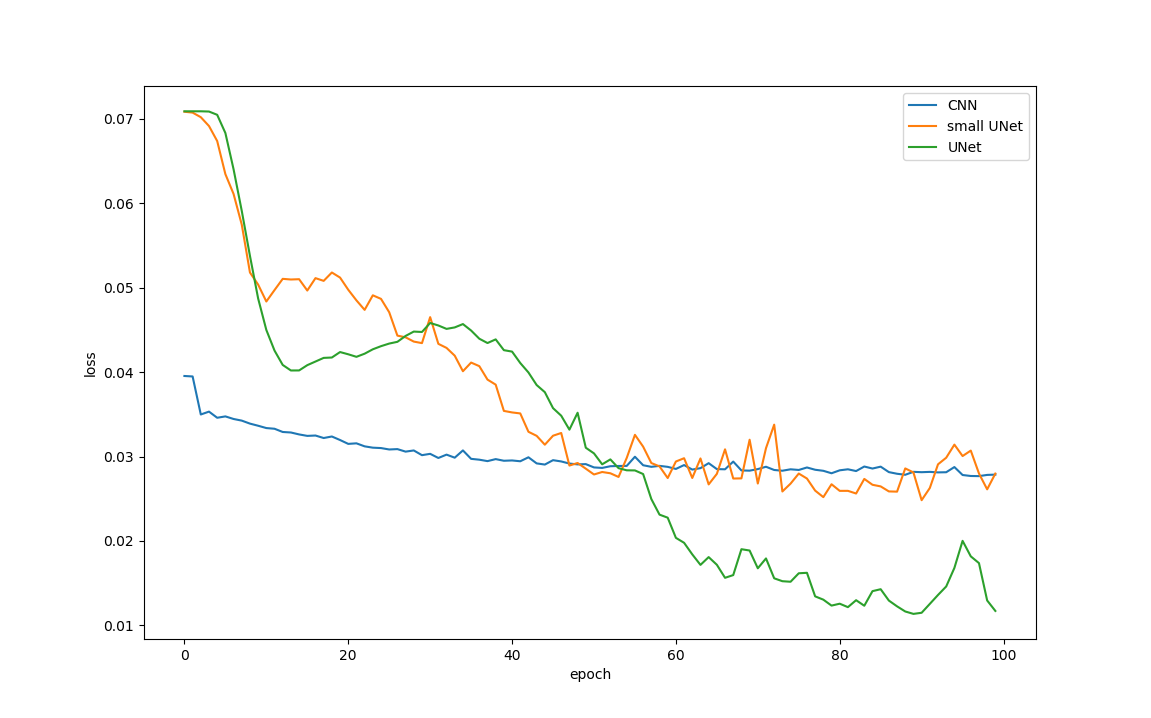
\includegraphics[width=\linewidth]{pics/Syntetische_Daten_CNN_UNet.png}
	\caption[Lernkurven verschiedener Architekturen auf Syntetische Daten]{Gezeigt ist die Lernkurve der Validierungsdaten auf 100 Epochen mit unterschiedlichen Netzarchitekturen. Die Verwendeten Trainingsdaten sind 1000 syntetische Bilder welche eine wandernde Regenfront Simulieren sollen. Das CNN ist etwa gleich gut wie das einfache UNet. Eine tiefere UNet Architektur (grün) erreicht eine noch bessere Performance. Die Architekturen sind in nachfolgenden Kapiteln genauer erläutert. }
	\label{imgCNNUNet}
\end{figure}

Die Abbildung \ref{imgCNNUNet} zeigt die Lernkurve der beiden Architekturen auf die Identische Problemstellung. Das UNet lernt in diesem Beispiel deutlich besser, weshalb die Vorhersage von Radarbildern in Zukunft mit einem UNet behandelt wird. Beide UNet Architekturen haben zu beginn eine deutlich schlechtere Vorhersage als das CNN, bereits nach 60 Epochen ist die einfache UNet Architektur gleich gut, während das grüne UNet die Performance sogar übertrifft und nach 100 Epochen die besten Ergebnisse liefert.
\newline
Die zweite Herangehensweise ist eine Klassifikation, hierbei geht es nicht darum das exakte Radarbild vorherzusagen, sondern einzuordnen, ob es Regnet oder nicht. Diese Aufgabe wurde als einfache Klassifikation für Konstanz, als auch als Pixelweise Klassifikation, für alle eingehenden Pixel durchgeführt. Für die Aufgabe der Klassifikation jedes Pixels wurde wieder ein UNet verwendet. Bei der Aufgabe der einfachen Klassifikation für Konstanz kamen beide Architekturen zum Einsatz.

\subsection{CNN}
\label{kapitelCNN}
Ein Convolutional Neural Networks im klassischen Sinne ist ein Netzwerk mit mehreren Convolutional-Layer, häufig in verbindung mit Pooling-Layer. Ein Convolutional-Layer besteht aus mehreren Filtern. Die Filter berechnen ein Output in abhängigkeit mehrerer Benachbarter 'Pixel' die größe der berücksichtigten Region hängt von der Filter- bzw. Kernelgröße ab.
Vorteile von Convolutional Layern sind zum einen, dass Nachbarschaften berücksichtigt werden, was gerade bei Bildern sehr sinnvoll ist, aber auch, dass der Speicherbedarf sehr gering ist, da nur eine kleine Anzahl an Gewichten für das Komplette Bild verwendet werden müssen.
Ein Pooling-Layer reduziert die Feature-Größe indem jeweils nur das stärkste Signal einer Region weitergegeben werden.

%MSE:
Für die Vorhersage der Radardaten haben wir uns für ein sehr einfaches CNN (Convolutional Neural Network) entschieden.
Als Eingabe erwartet es mehrere Zeitschritte um darauf eine Vorhersage zu treffen. Der input ist also dreidimensional wobei die dritte dimension die Zeitschritte und die anderen Dimensionen die Bildauflösung beschreiben. Die Eingabe wird durch sechzehn Convolution Kernel der Größe 5x5 verrechnet. Anschließend folgen zweiunddreißig weitere 5x5 Kernel. Anschließend ist ein optionales Dropout Layer eingebunden, welches nur zu Testzwecken verwendet wurde. Die Performance hatte sich dadurch aber nicht bemerkenswert verändert. Abschließend kommt ein Kernel, welcher die nun entstandenen Features zu einem Bild zusammenfasst. Hierzu wird ein 3x3 Kernel verwendet. Alle Layer sind mit einer ReLu als Aktivierungsfunktion ausgestattet.
Die Performance ist weniger gut, als ein UNet kann aber mit der sehr einfachen UNet Architektur mithalten. Zu sehen ist das in Abbildung \ref{imgCNNUNet} wo die Blaue Kurve dem Lernverhalten der hier beschriebenen CNN Architektur entspricht.

%Klassifikation:
Für Klassifikation des Konstanzpixels entschlossen wir uns dazu das CNN welches wir eingangs verwendet hatten um den MNIST Datensatz zu lernen wieder zu verwenden. Dieses Netz besteht lediglich aus zweiunddreißig 3x3 Kerneln mit ReLu aktivierungsfunktion. Anschließend folgt ein 2x2 MaxPooling und ein Flatten Layer. Die nun \gqq{flachen} Daten werden durch ein FullyConnected Layer auf 30 Neuronen reduziert. Darauf folgt ein Dropout Layer mit 20\% welches Overfitting verhindern soll. Abschließend Folgt ein Layer das die Features auf drei ausgabe Neuronen verrechnet. Damit die Klassifizierung einfacher zu interpretieren ist, wird als aktivierungsfunktion ein SoftMax verwendet.

\subsection{UNet}
\label{kapitelUNet}
%was ist ein Unet?
Ein Unet ist eine spezielle Form eines CNN. Es hat seinen Namen durch die 'U-Förmige' Architektur, siehe Abbildung \ref{imgUNetA}
\begin{figure}[h]
	\centering
	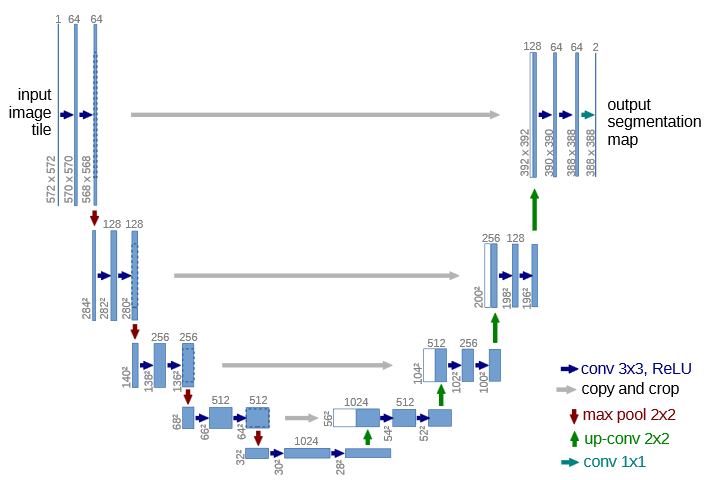
\includegraphics[width=\linewidth]{pics/UNet_Biomedical}
	\caption[UNet aus Paper von O. Ronneberger, P. Fischer und T. Brox]{Die hier abgebildete Architektur entstammt dem Paper zur Biomedizinischen Bildsegmentierung \cite{DBLP:journals/corr/RonnebergerFB15}. Hier abgebildet ist eine Typische UNet-Architektur, welche von den Eingabebildern (oben Links) zu der Ausgabe (oben Rechts) die Features stets verkleinert (rote Pfeile) und im späteren verlauf auch wieder vergößert (grüne Pfeile). Da bei dem wieder vergrößern der Daten nicht alle Informationen wiedergewonnen werden können, gibt es auch Querverbindungen (graue Pfeile) welche die zuvor errechneten Features an ein späteres Layer weitergibt.}
	\label{imgUNetA}
\end{figure}

Das Unet besteht aus mehreren Convolutional Layern, mit anschließendem Pooling. Hierdurch wird die Featuregröße immer weiter Reduziert. Ab einem bestimmten Punkt wird die Featuregröße wieder aufgeblasen, um schlussendlich am output die gleiche Größe wie am Input zu besitzen. Beim 'aufblasen' kommt ein Upsampling Layer zum Einsatz. Da allerdings beim vergrößern der Features nicht alle Informationen wiederhergestellt werden können gibt es auch noch horizontale Verbindungen, durch welche zuvor erstellte Features später weiterverwendet werden können.
Diese Architektur ist sehr ähnlich zu einem Autoencoder und wurde erstmals für biomedizinische Zwecke verwendet. Da sich mit dieser Architektur mehrere Bilder einlesen und auch beliebig viele Bilder ausgeben lassen, versuchen wir damit die Wettervorhersage für mehrere Zeitschritte zu lösen.

%Einstiegsnetz
Um eine geeignete Architektur auszuwählen haben wir ein einfaches Testszenario aufgebaut, welches unterschiedliche Netzarchitekturen zu lösen hatten. Die hierfür verwendeten Daten waren aus jeweils 100x100x5 Pixeln großen Syntetischen Daten aufgebaut.
ToDo: Syntetische Daten erklären.
Das erste U-Net besteht aus lediglich einem Upsamling Layer. Die Architektur sieht wie folgt aus:
Eingangs verarbeiten zweiunddreißig 5x5 Convolutional Layer mit Padding die Eingabe. Diese wird über ein 3x3 MaxPooling reduziert. Die Reduzierten Daten werden durch ein 3x3 Upsampling wieder in die ursprüngliche Größe zurück gewandelt und mit den Features vor dem MaxPooling verbunden. Die so entstehenden 100x100x64 Features werden anschließend über einen 1x1 Convolutional Layer zu einem Ausgabebild zusammengefasst.
Die zu diesem Netz gehörende Lernkurve ist in Abbildung \ref{imgCNNUNet} zu sehen. Die Performance unterscheidet sich kaum zu der eines Klassischen CNNs. Daher versuchen wir die Architektur tiefer zu gestalten.

%Unet64
Das finale UNet wie es in Abbildung \ref{imgCNNUNet} in grün zu sehen ist besteht aus mehreren Ebenden.
Zunächst wird die Eingabe durch ein Convolutional-Layer mit zehn 3x3 Kerneln und anschließender ReLU als Aktivierungsfunktion geleitet. Die so entstehenden Features werden als Conv01 bezeichnet und später wieder verwendet.
Die Features werden anschließend durch ein MaxPooling-Layer der Größe 2x2 verkleinert. Anschließend folgt ein weiteres Convolutional-Layer mit zwanzig 3x3 Kerneln. diese Features werden im weiteren als Conv02 bezeichnet.
Auch hierauf folgt wieder ein 2x2 MaxPooling-Layer mit anschließend einem weiteren Convolutional-Layer mit zwanzig Kerneln der größe 3x3. Diese Features werden als Conv03 weiterverwendet.
Die tiefste Ebene in dieser Architektur besteht wieder aus einem Convolutional-Layer mit zwanzig Kerneln der größe 3x3. Auch hier folgt ein 2x2 MaxPooling. Diese Features heißen Conv04.
Ab nun werden die Features wieder größer. Ein Upsamling-Layer der Größe 2x2 sorgt dafür, dass die Features mit den zuvor erstellten Conv04 Features verbunden werden können. dies geschieht durch ein Concatenate-Layer, was die beiden Tensoren zu einem größeren verbindet. Die so entstandenen Features werden wieder durch ein Upsampling-Layer der größe 2x2 vergrößert und mit den Conv03 Features verbunden. Auch diese Daten werden wieder über ein Upsampling-Layer der größe 2x2 verrechnet und anschließend mit den Conv02 Features verbunden. Abschließend werden die Daten durch ein weiteres 2x2 Upsampling-Layer verrechnet und mit den Conv01 Features verbunden. Abschließend kommt ein als ausgabe ein Convolutional-Layer mit einem 1x1 Kernel der alle Features zu einem Graustufenbild zusammenfasst.
Alle Hier erwähnten Convolutional-Layer haben eine ReLU als aktivierungsfunktion, wodurch negative Werte ausgeschlossen werden. Des weiteren besitzen diese Layer auch Padding um die Bildgröße beizubehalten.

Alle oben genannten Architekturen werden mit dem Adam optimizer Trainiert. Je nach Aufgabenstellung dient als Fehlerfunktion der MSE, beim Vorhersagen der Radardaten, oder die Categorical Cross-Entropy, beim lösen des Klassifikationsproblems.
